Boehringer Ingelheim ist ein bekannter Name in der Pharmabranche. Das Unternehmen gehört weltweit zu den 20 größten Pharmaunternehmen. Mit einem klaren Schwerpunkt auf Humanpharma und Tiergesundheit hat es sich in diesen Bereichen fest etabliert.
Gegründet im Jahr 1885, ist Boehringer Ingelheim über die Jahre stark gewachsen und beschäftigt heute rund 53.500 Mitarbeitende.
Boehringer Ingelheim zählt zu den weltweit führenden Anbietern im Bereich Tiergesundheit. Den starken Marktstand verdankt das Unternehmen insbesondere seinem breiten Portfolio an Produkten und Dienstleistungen. Dieses Engagement für Tiergesundheit unterstreicht die Mission von Boehringer Ingelheim, Gesundheit und Wohlbefinden in allen Lebensphasen zu verbessern.
\ac{ACID} steht für Atomicity, Consistency, Isolation und Durability.
\citep{boehringerProfile2024}.
\begin{figure}[H]
    \centering
    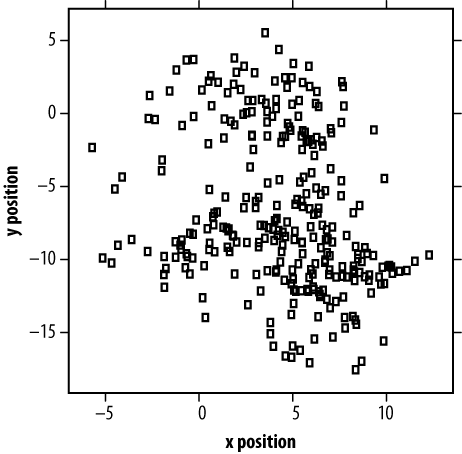
\includegraphics[width=0.45\textwidth]{Abbildungen/01_example_image.png}
    \caption{Lage der Standorte im x/y‑Koordinatensystem}
    \label{fig:figure1}
\end{figure}
Beispiel
\begin{table}[H]
    \centering
    \begin{tabular}{|l|l|l|p{5cm}|}
        \hline
        \textbf{Name} & \textbf{Ring} & \textbf{Quadrant} & \textbf{Beschreibung}          \\
        \hline
        Babel         & adopt         & tools             & JavaScript‑Compiler für ES6+. \\
        \hline
        Apache Kafka  & trial         & tools             & Event‑Streaming‑Plattform.     \\
        \hline
        Bug bounties  & trial         & techniques        & Belohnungen für das Finden von Sicherheitslücken.     \\
        \hline
    \end{tabular}
    \caption{Beispieltabelle mit 3 Technologien}
    \label{tab:my_label}
\end{table}